% Template for ICIP-2022 paper; to be used with:
%          spconf.sty  - ICASSP/ICIP LaTeX style file, and
%          IEEEbib.bst - IEEE bibliography style file.
% --------------------------------------------------------------------------
\documentclass{article}
\usepackage{spconf,amsmath,graphicx}
\usepackage{booktabs}
\usepackage{xeCJK}

\setCJKmainfont{HaranoAjiMincho-Regular.otf}

% \setCJKmainfont{Noto Serif CJK JP}       % Default CJK font (Japanese)
% \setCJKfamilyfont{zh_sim}{Noto Serif CJK SC} % Font family for Simplified Chinese
% \setCJKfamilyfont{zh_tra}{Noto Serif CJK TC} % Font family for Traditional Chinese

% 3. Create short commands to switch Chinese variants easily
\newcommand{\simplified}[1]{{\CJKfamily{zh_sim}#1}}
\newcommand{\traditional}[1]{{\CJKfamily{zh_tra}#1}}

\usepackage{tikz}
\usetikzlibrary{arrows.meta,positioning,decorations.pathreplacing}

% Example definitions.
% --------------------
\def\x{{\mathbf x}}
\def\L{{\cal L}}

% Title.
% ------
\title{Boundary-Free Contextual Biasing: Depth-Adaptive Gating and Reading-Space Matching for Unsegmented Languages}
%
% Single address.
% ---------------
\name{Muhammad Huzaifah, Yu Pan, Zachary Yeo, Ningjie Bai, Guangzhao Yang}  %\thanks{Thanks to XYZ agency for funding.}
\address{R\&D Team, Recho Inc., Tokyo, Japan}
%
% For example:
% ------------
%\address{School\\
%	Department\\
%	Address}
%
% Two addresses (uncomment and modify for two-address case).
% ----------------------------------------------------------
%\twoauthors
%  {A. Author-one, B. Author-two\sthanks{Thanks to XYZ agency for funding.}}
%	{School A-B\\
%	Department A-B\\
%	Address A-B}
%  {C. Author-three, D. Author-four\sthanks{The fourth author performed the work
%	while at ...}}
%	{School C-D\\
%	Department C-D\\
%	Address C-D}
%
\begin{document}
\ninept
%
\maketitle
%
\begin{abstract}
Contextual biasing supplies an ASR system with a list of expected words at inference time, but existing methods rely on word boundaries that Japanese and Chinese do not provide. We present a boundary-free biasing decoder for frozen public CTC models, built on a character-level Aho–Corasick automaton, with no training and no second pass. Two evidence-based mechanisms replace the boundary: a depth-adaptive gate that sets how hard to push from match depth, and reading-space matching for when the audio is right but the characters are wrong. On Aishell-1 NE's hard R1 subset we reach 66.5\% recall, above the trained CLAS baseline (64\%), transferring to WenetSpeech and to a second architecture without retuning. We release the first open Japanese contextual-biasing benchmark, where biasing lifts rare-word recall by 25 points at precision above 97\%, and still by 19 and 22 points against 1,000-word lists.
\end{abstract}
%
\begin{keywords}
contextual biasing, automatic speech recognition, CTC, greedy decoding, unsegmented languages
\end{keywords}
%
\section{Introduction}
\label{sec:intro}

Even strong automatic speech recognition (ASR) models reliably miss the vocabulary their users care most about -- names, product terms, domain jargon -- rare in training data yet often carrying the utterance's meaning. \textit{Contextual biasing} addresses this with auxiliary information. A list of likely words (\textit{hotwords}) is supplied at inference and the decoder steered toward them. In production, models are frozen and lists can change per request, so steering must happen at decode time. A tight latency budget further rules out beam search and second-pass rescoring, leaving a single greedy pass over the CTC \cite{ctc} frame-synchronous token stream.

Any biasing decoder must decide, at every frame, where a listed word can start, whether the hypothesis is inside one and how far, and in what representation the match is scored. Segmented languages answer all three with one signal, the word boundary plus a stable written form, and most biasing literature is built on it \cite{aleksic15_interspeech,zhao19d_interspeech,sun2021tree,context_trie,andrusenko2025turbobias}. Unsegmented languages like Japanese (JA) and Chinese (ZH) answer none. First, no boundary token exists in the CTC stream, so every character position is a potential word entry. Second, no unit above the character is stable. The same string tokenizes context-dependently, so a listed word has no fixed token sequence, and CJK homophony means the model can decode the audio correctly and still emit the wrong characters (e.g. 照会→紹介). The stable object is the reading, which straddles token boundaries structurally. Matching must therefore run below the token, on characters at the surface and on morae or syllables in reading space. This buys no accuracy on its own (they tie in our experiments), but it makes the boundary's two lost roles recoverable. How hard to push follows from per-character match depth, which our gate switches on; what the push anchors to is the listed surface by default and, where homophony blocks it, per-mora or per-syllable reading state. Neither quantity exists at the word or token level.

No prior system exposes either quantity. Trained biasing attaches a module to the model (CLAS \cite{pundak2018deep}, TCPGen \cite{sun2021tree}, CB-Conformer \cite{xu2023cb}, SeACo-Paraformer \cite{shi2024seaco}); the ZH systems score each hotword as one learned embedding, leaving no incremental match state, at the cost of training data, model surgery and a fixed list distribution. Likewise phonetic biasing exists only at training time \cite{bruguier2019phoebe,chen2019joint} or as prompting \cite{peng24b_interspeech}; none runs a reading-space automaton on an unmodified checkpoint. Decode-time methods bypass training but anchor entries on boundaries and retune per list at scale \cite{aleksic15_interspeech,zhao19d_interspeech,context_trie,andrusenko2025turbobias}. For JA, WCTC-Biasing \cite{nakagome25_interspeech} is retraining-free but needs model-internal access, and its lists are error-mined from evaluation sets and unreleased. Open biasing sets exist for EN \cite{context_trie} and ZH \cite{xu2023cb,shi2024seaco,wang2025contextasr}, but not JA.


% No prior system exposes either quantity, for different reasons in each line of work. Trained biasing attaches a module to the model, such as attention over the list (CLAS [6]), tree-constrained pointer generators (TCPGen [9]), biasing layers (CB-Conformer [11]), or hotword attention in NAR systems (SeACo-Paraformer [12]). The ZH systems [11, 12] do reach unsegmented text, but by removing the need for a boundary rather than replacing it: each hotword is encoded into a single vector (an embedding layer in [11]; a shared embedding + LSTM in [12]) and scored by attention against decoder or encoder states, so no incremental match state exists to anchor and the three questions are absorbed into training. The cost is hotword-supervised training data, model surgery, a list distribution fixed at training time, and no decode- time control surface. Decode-time biasing does not require training, whether on-the-fly rescoring and shallow fusion [3--5], trie/WFST deep biasing [10], CTC word spotting [20], or GPU phrase-boosting trees (TurboBias [13], streaming follow-up [23]), but it is built on boundary-anchored word entries and, at scale, per-list retuning ([13] retunes its boost weight with list size; we quantify why in [section]). Phonetic biasing exists only at training time, as pronunciation-aware CLAS (Phoebe [7]) and joint grapheme-phoneme embeddings [8], or as prompting (OWSM v3.1 [15]); none runs a reading-space automaton at decode time on an unmodified checkpoint. For JA, retraining-free biasing exists via wildcard-CTC keyword spotting (WCTC-Biasing [24]), but it requires model-internal access and its keyword lists, mined from the system's own errors on the evaluation sets, are not released. Open biasing evaluation sets exist for EN [10] and ZH [11, 12, 25], none for JA.

Our contributions are as follows: (1) A depth-adaptive biasing gate whose two extremes, restricting bias to the model's top-K candidates and letting it re-choose without a cap, are endpoints of one family switched by match-evidence depth in per-character information units. (2) Decode-time reading-space biasing, where the automaton advances on dictionary readings while bias promotes the listed surface, fused with the surface automaton by a correlation-discount rule. (3) The first open Japanese contextual-biasing benchmark, from JSUT \cite{sonobe2017jsut} and Common Voice JA \cite{ardila2020common}, stratified by hotword length and script (full construction methodology in a companion paper). (4) A cross-regime analysis on two architectures \cite{an2024funaudiollm,peng24b_interspeech} and two languages, characterizing failure modes on three axes: the threshold on script, the weight on list scale, and the cap on tokenizer granularity, and that one adaptive setting per language is robust across all of them.


%showing why unbounded gates are fragile on three independent axes and bounded gates are not.


% Our contributions are as follows. (1)~A depth-adaptive biasing gate whose two published extremes -- restricting bias to the model's top-K candidates, and letting it re-choose without a cap -- are endpoints of one family, switched by match-evidence depth in per-character information units. At the parents' own weight, one setting matches the best tuned parent within 1pp across scripts and list sizes without collapsing; weight, not gate, is the axis needing per-scale tuning. (2)~Decode-time reading-space biasing, where hotwords become mora or syllable paths, tokens advance by dictionary readings, and bias promotes the corresponding character surface, fused with the surface automaton in a single pass by a correlation-discount rule. (3)~The first open Japanese contextual-biasing benchmark, from JSUT [18] and Common Voice JA [19], stratified by hotword length and script, the regime variables our analysis identifies (construction methodology in a companion paper). (4)~A cross-regime analysis on two architectures and two languages showing why unbounded gates are fragile on three independent axes and bounded gates are not.

\section{Method}
\label{sec:method}

\subsection{Boundary-free surface biasing}
Hotwords are compiled into a character-level Aho–Corasick automaton \cite{aho-corasick}, a trie over the hotword set plus failure links to the longest matched suffix that is also a hotword prefix (Fig.~\ref{fig:automaton}a). It reports every occurrence in one left-to-right pass at a per-frame cost independent of list size. Because decoding emits tokens rather than characters, the automaton is precomputed into two token-level tables giving, for each state and token, the bias accrued by walking that token's surface and the state it reaches (Fig.~\ref{fig:automaton}b); a multi-character piece therefore crosses several edges in one emission. Decoding stays ordinary greedy CTC. At each frame the bias row $b(q_t,\cdot)$ is added to the log-probabilities $\ell_t$ and the emitted token $v_t$ advances the state, costing one row lookup, one transition and one integer register per stream, batched and streaming-compatible. Writing $d(q)$ for the depth of state $q$, its distance from $q_0$ and hence the number of characters matched so far, a state carries potential $\psi(d)=w\sum_{i=1}^{d}(2+\ln i)$, and a token moving the automaton from $q$ to $q'$ accrues $\psi(d(q'))-\psi(d(q))$ plus a lump on completing a hotword, as in \cite{andrusenko2025turbobias} but over characters. Credit therefore grows with match depth, the single weight $w$ scales the whole schedule, and negative deltas are clamped so abandoning a partial match is free. The failure links make every character position a possible entry, the boundary-free property, and let partial matches collapse without corrupting the hypothesis.

%Match scoring gives per-character advancement credit plus a completion lump, as in \cite{andrusenko2025turbobias} but over characters. 

%scaled by a single global weight $w$ that sets the bias magnitude, with negative deltas clamped so abandoning a partial match is free. 
% It reports every occurrence in one left-to-right pass at a cost independent of list size. 

% Match scoring uses potential-style credit, as in [13] but over characters, giving per-character advancement plus a completion lump, with negative deltas clamped so abandoning a partial match is free (charging for it was measured and rejected, §5)



\subsection{Depth-adaptive gating}

The gate replaces the boundary's control role, deciding how hard to push from the evidence the partial match carries. Two mechanisms bound the design space. The first, \textit{masked biasing}, is ours. Bias is added only among the model's top-K tokens before the argmax; making explicit a restriction beam search obtains from pruning \cite{zhao19d_interspeech}, it is entry-safe but unable to rescue a continuation ranked below K. The second, \textit{two-stage} (following TurboBias's greedy semantics \cite{andrusenko2025turbobias}, source-verified), re-chooses without a cap among candidates other than blank and the previous token; powerful far into a match but catastrophic at entries, where dense unmarked candidates let strong bias hijack ordinary text. Each fails outside its band (§4.3). A boundary supplies that distinction at zero depth, and \cite{zhao19d_interspeech} obtains it from word prefixes; without either, we infer it from match evidence.

%Beam search obtains this restriction accidentally from pruning, a defect [5] removes by biasing before pruning. Greedy decoding has no beam, so we impose it deliberately as the safety mechanism. It is entry-safe but capped far into a match, unable to rescue a continuation ranked below K. 




\begin{figure}[t]
\centering

%% ================= (a) character automaton =================
\begin{tikzpicture}[
  >={Stealth[round]}, font=\small,
  st/.style={circle,draw,minimum size=7.2mm,inner sep=0pt},
  ac/.style={st,double,double distance=0.5pt}]

  \node[font=\footnotesize\bfseries] at (-1.15,0.0) {(a)};

  \node[st] (q0) at (0,0)      {$q_0$};
  \node[st] (q1) at (1.50,0)   {$q_1$};
  \node[ac] (q2) at (3.00,0)   {$q_2$};
  \node[st] (q3) at (1.50,-1.1){$q_3$};
  \node[ac] (q4) at (3.00,-1.1){$q_4$};

  % edges on the 東京都 walk are drawn thick and numbered by input position
  \tikzset{stp/.style={circle,draw,inner sep=0.4pt,font=\tiny,fill=white}}
  \draw[->,thick] (q0) -- node[above=-1pt]{東} node[below=2pt,stp]{1} (q1);
  \draw[->,thick] (q1) -- node[above=-1pt]{京} node[below=2pt,stp]{2} (q2);
  \draw[->]       (q0) -- node[below=-1pt,pos=0.55]{京} (q3);
  \draw[->,thick] (q3) -- node[above=-1pt]{都} node[below=2pt,stp]{3} (q4);
  \draw[->,dashed,thick] (q2) -- node[fill=white,inner sep=1pt,font=\scriptsize,pos=0.38]{fail} (q3);

  \node[anchor=west,font=\scriptsize] at (3.45,0)    {accept 東京};
  \node[anchor=west,font=\scriptsize] at (3.45,-1.1) {accept 京都};

\end{tikzpicture}

\vspace{2mm}

%% ========= (b) precomputed table + per-frame flow =========
\begin{tikzpicture}[
  >={Stealth[round]}, font=\small,
  bx/.style={draw,rounded corners=1pt,inner sep=2pt,font=\scriptsize}]

  \node[font=\footnotesize\bfseries] at (-1.15,0.0) {(b)};

  % flow row (y = 0)
  \node                            (lg)   at (0.00,0) {$\ell_t$};
  \node[circle,draw,inner sep=1pt] (plus) at (0.98,0) {$+$};
  \node[bx]                        (am)   at (2.20,0) {$\arg\max$};
  \node                            (vt)   at (3.20,0) {$v_t$};
  \draw[->] (lg)   -- (plus);
  \draw[->] (plus) -- (am);
  \draw[->] (am)   -- (vt);

  % single precomputed table, cells = (bias, next state)
  \node[bx] (tab) at (1.78,-1.35) {%
    \begin{tabular}{c|cc}
      $q$   & 東                & 京都                        \\\hline
      $q_0$ & $2.00,\;q_1$      & $4.69{+}c,\;q_4$            \\
      $q_1$ & $0,\;q_1$         & $2.69{+}2c,\;q_4$           \\
    \end{tabular}};

  \draw[->] (tab.north -| plus) -- node[left,font=\scriptsize,inner sep=1pt]{$b(q_t,\cdot)$} (plus.south);
  \draw[->] (vt.south) -- node[right,font=\scriptsize,inner sep=1pt]{$q_{t+1}$} (tab.north -| vt);
\end{tikzpicture}

\caption{(a) Character-level Aho-Corasick automaton for 東京 and 京都; solid arrows are trie edges, the dashed one a failure link. Circled numbers trace the decoded stream 東京都 along the thick path, the failure link moving from the end of 東京 into the middle of 京都 without consuming a character, so both are matched. (b) The precomputed token-level table and per-frame decode flow; cells give the state reached and the bias $\psi(d')-\psi(d)$ at $w{=}1$, plus a lump $c$ per hotword completed.
}
\label{fig:automaton}
\end{figure}

% \begin{figure}[t]
% \centering

% %% ================= (a) character automaton =================
% \begin{tikzpicture}[
%   >={Stealth[round]}, font=\small,
%   st/.style={circle,draw,minimum size=7.2mm,inner sep=0pt},
%   ac/.style={st,double,double distance=0.5pt}]

%   \node[font=\footnotesize\bfseries] at (-1.15,0.0) {(a)};

%   \node[st] (q0) at (0,0)      {$q_0$};
%   \node[st] (q1) at (1.50,0)   {$q_1$};
%   \node[ac] (q2) at (3.00,0)   {$q_2$};
%   \node[st] (q3) at (1.50,-1.1){$q_3$};
%   \node[ac] (q4) at (3.00,-1.1){$q_4$};

%   % edges on the 東京都 walk are drawn thick and numbered by input position
%   \tikzset{stp/.style={circle,draw,inner sep=0.4pt,font=\tiny,fill=white}}
%   \draw[->,thick] (q0) -- node[above=-1pt]{東} node[below=2pt,stp]{1} (q1);
%   \draw[->,thick] (q1) -- node[above=-1pt]{京} node[below=2pt,stp]{2} (q2);
%   \draw[->]       (q0) -- node[below=-1pt,pos=0.55]{京} (q3);
%   \draw[->,thick] (q3) -- node[above=-1pt]{都} node[below=2pt,stp]{3} (q4);
%   \draw[->,dashed,thick] (q2) -- node[fill=white,inner sep=1pt,font=\scriptsize,pos=0.38]{fail} (q3);

%   \node[anchor=west,font=\scriptsize] at (3.45,0)    {accept 東京};
%   \node[anchor=west,font=\scriptsize] at (3.45,-1.1) {accept 京都};

% \end{tikzpicture}

% \vspace{2mm}

% %% ========= (b) precomputed table + per-frame flow =========
% \begin{tikzpicture}[
%   >={Stealth[round]}, font=\small,
%   bx/.style={draw,rounded corners=1pt,inner sep=2pt,font=\scriptsize}]

%   \node[font=\footnotesize\bfseries] at (-1.15,0.0) {(b)};

%   % flow row (y = 0)
%   \node                            (lg)   at (0.00,0) {$\ell_t$};
%   \node[circle,draw,inner sep=1pt] (plus) at (0.98,0) {$+$};
%   \node[bx]                        (am)   at (2.20,0) {$\arg\max$};
%   \node                            (vt)   at (3.20,0) {$v_t$};
%   \draw[->] (lg)   -- (plus);
%   \draw[->] (plus) -- (am);
%   \draw[->] (am)   -- (vt);

%   % single precomputed table, cells = (bias, next state)
%   \node[bx] (tab) at (1.78,-1.35) {%
%     \begin{tabular}{c|cc}
%       $q$   & 東                & 京都                        \\\hline
%       $q_0$ & $2.00,\;q_1$      & $4.69{+}c,\;q_4$            \\
%       $q_1$ & $0,\;q_1$         & $2.69{+}2c,\;q_4$           \\
%     \end{tabular}};

%   \draw[->] (tab.north west) -- node[left,font=\scriptsize,inner sep=1pt]{$b(q_t,\cdot)$} (plus.south);
%   \draw[->] (vt.south) -- node[right,font=\scriptsize,inner sep=1pt]{$q_{t+1}$} (tab.north east);
% \end{tikzpicture}

% \caption{(a) Character-level Aho--Corasick automaton for the hotwords 東京 and 京都;
% solid arrows are trie edges, the dashed arrow a failure link. Circled numbers
% trace the decoded character stream 東京都 along the thick path; the failure
% link moves the automaton from the end of 東京 into the middle of 京都 without
% consuming a character, so both listed strings are matched. (b) The precomputed
% token-level table, whose cells give the bias accrued and the state reached,
% and the per-frame decode flow. Cells give $\psi(d')-\psi(d)$ at $w{=}1$ plus a
% completion lump $c$ for each hotword the token finishes; 京都 from $q_1$
% completes both.}
% \label{fig:automaton}
% \end{figure}

Let $d_t=d(q_t)$ be the depth of the current state, $S=\{\emptyset, v_{t-1}\}$ the non-emitting set (blank or repeat token), $\hat{v}_t = \arg\max_v \ell_t(v)$ the unbiased proposal, and $\tilde{b}_t(v) = b_t(v)\mathbf{1}[v \in \text{top-}K(\ell_t)]$ the masked bias. The threshold $d^\star$ splits matches into \textit{entry} and \textit{deep} bands, and the gate assigns each mechanism to its own, replacing the argmax of Fig.~\ref{fig:automaton}b:

% Let $d_t = d(q_t)$ be the match depth at frame $t$ (distance from $q_0$ in Fig.~\ref{fig:automaton}a), $b_t(v) = b(q_t,v)$ the bias row for the current state, $S = \{\emptyset,\, v_{t-1}\}$ the non-emitting set (blank or a repeat of the previous token), and $\hat{v}_t = \arg\max_v \ell_t(v)$ the unbiased proposal. The masked bias is $\tilde{b}_t(v) = b_t(v)\,\mathbf{1}\!\left[v \in \text{top-}K(\ell_t)\right]$. The depth-adaptive gate assigns each mechanism to its band, replacing the single argmax of Fig.~\ref{fig:automaton}b:


\begin{equation*}
v_t =
\begin{cases}
\arg\max_v \left[\ell_t(v) + \tilde{b}_t(v)\right], & d_t < d^\star\\[3pt]
\hat{v}_t, & d_t \ge d^\star,\ \hat{v}_t \in S\\[3pt]
\arg\max_{v \notin S} \left[\ell_t(v) + b_t(v)\right], & \text{otherwise}
\end{cases}
\end{equation*}

This gives entry/insertion control below $d^\star$ and traversal protection above it. Setting $d^\star$=$\infty$ recovers masked biasing and $d^\star$=0 recovers two-stage, so $d^\star$ parameterizes the family containing both. Counting depth in raw characters would leave $d^\star$ script-dependent: a Han character carries $\approx$$1.75\times$ a kana's unigram surprisal on the benchmark transcripts, so we weight Han 1.0, kana 0.5 (unrounded 0.57 gives identical decodes) and threshold in Han-equivalent units. This is identical to character counting on uniform-script lists (ZH, verified byte-identical); on mixed scripts it replaces the separate kanji and kana optima with a single threshold $d^\star$=3 on the JA benchmark (§4.3).

%given a Han character carries about 1.75$\times$ the unigram surprisal of a kana on the benchmark transcripts (11.4 vs 6.5 bits), we weight Han 1.0 and kana 0.5, (unrounded 0.57 gives identical decodes)


\subsection{Reading-space biasing}
A calibrated surface push cannot help when the error is orthographic. The hypothesis carries the right reading in the wrong characters, and the surface automaton never engages (紹$\neq$照 at entry). We therefore run a second automaton in reading space. Offline, each hotword becomes a kana (MeCab/UniDic\footnote{https://taku910.github.io/mecab/}) or pinyin (tone-less pypinyin\footnote{https://github.com/mozillazg/python-pinyin}) path; each vocabulary token is assigned its candidate readings; and an alignment maps each surface character to its reading span. At decode time the automaton advances on any homophone token, anchoring on what the audio supports, while bias is spent only on the listed surface's tokens, an asymmetric match/push applied under the same top-K gate. It requires no runtime lexicon or trained module, and adds one further row lookup, transition and register per frame. It is the decode-time counterpart of \cite{bruguier2019phoebe,chen2019joint}, and distinct from prompting \cite{peng24b_interspeech}.

Because any homophone advances a reading match, each word's push is damped by $1/\bigl(1 + \log_{10}(1+f)\bigr)$, with $f$ its reading's
frequency in an independent corpus (ReazonSpeech transcripts \cite{yin2023reazonspeech} for JA, Aishell-1 training transcripts \cite{bu2017aishell} for ZH, eval split excluded); the list's per-word weight expresses domain intent. Both automata can run in a single greedy loop with biases combined pre-argmax. They are correlated evidence, so summing double-counts shared spans while the max under-credits corroboration; we fuse the surface and reading credits $s$ and $r$ as $\max(s,r) + \lambda \min(s,r)$, where $\lambda$ discounts the weaker source's corroboration for that correlation, $\lambda$=0 giving pure max and $\lambda$=1 pure sum. Gate evidence is unified in entropy units, so §2.2's gate applies unchanged.


\section{Open JA biasing benchmark}




The only JA biasing evaluation we know of \cite{nakagome25_interspeech} mines its keyword lists by decoding the evaluation sets with the model under test, which is circular by construction, and does not release them; the recent large contextual benchmark \cite{wang2025contextasr} covers ZH and EN only. We therefore construct and release the first open JA contextual-biasing evaluation set, built model-free from JSUT basic5000 \cite{sonobe2017jsut} and Common Voice (CV) 26 ja \cite{ardila2020common}. Model-free construction means the set is not easier for any particular system, unlike error-mined lists. 

\begin{table}[htb]
\centering
\caption{JA biasing benchmark statistics. JSUT is fully human-verified; CV is partly human-reviewed, the unreviewed residual noise rate is measured by a seeded blind sample and reported in the dataset card.}
\label{tab:bench}
\footnotesize
\setlength{\tabcolsep}{4.5pt}
\begin{tabular}{lrrrr}
\toprule
corpus & utts & w/ target & hotwords & occurrences \\
\midrule
JSUT     & 5,000   & 422 (8.44\%)    & 477   & 489    \\
CV ja & 300,077 & 25,876 (8.62\%) & 4,357 & 27,108 \\
\bottomrule
\end{tabular}
\end{table}


Because Japanese is unsegmented, the first question is what counts as a word. We annotate lexical-unit spans with MeCab/UniDic and merge compounds only where the merged form is itself corpus-attested, which keeps words like 東京大学 whole without absorbing the phrase around it. Target spans are formed after proper noun and rare-word filtering, followed by native-speaker screening. They are matched as annotated spans rather than substring hits, so a listed word occurring inside a longer word never counts. Per-utterance lists at $N \in \{100, 500, 1000, 2000\}$ fill with distractor words mined from Wikipedia, checked so that no distractor appears in its own utterance's reference and sampled to each corpus's target length profile, which keeps surface statistics from separating targets from distractors. The two corpora are complementary. JSUT is small, read and fully verified, while Common Voice contributes nearly two orders of magnitude more occurrences from crowd-sourced speech at the cost of a partially screened tail. Targets are labeled by length (2–6+ characters) and script, the regime variables analyzed in §4.3, made into a design principle. We release the per-utterance lists, span annotations, verification suite and card, seed-deterministic; audio remains under the source corpora's licenses. A more complete treatment of the methodology is planned for a companion resource paper.

% Targets are annotated span surfaces rather than substring hits, so a listed word inside a longer word never counts. Per-utterance lists at $N \in \{100, 500, 1000, 2000\}$ draw distractors from a shared leak-checked Wikipedia-mined pool matched to each corpus's target profile. Targets are labeled by length (2–6+ characters) and script, the regime variables analyzed in §4.3, made into a design principle. We release the per-utterance lists, span annotations, verification suite and card, seed-deterministic; audio remains under the source corpora's licenses. A more complete treatment of the methodology is planned for a companion resource paper.



\section{Experiment and results}

\subsection{Experimental setup}
We use two frozen public checkpoints, SenseVoice-small \cite{an2024funaudiollm} with a single-character CJK vocabulary and OWSM-CTC \cite{peng2024owsm} with multi-character BPE pieces, decoded with greedy CTC throughout. On ZH we evaluate Aishell-1 \cite{bu2017aishell} NE under the SeACo protocol \cite{shi2024seaco}, tuned on dev and reported on test, and WenetSpeech contextual set \cite{zhang2022wenetspeech} released with CB-Conformer \cite{xu2023cb} (298 words, 22k utterances), used untuned as a transfer cell. On JA, we evaluate §3, with a configuration frozen on an internal development set, barring $d^\star$=3, chosen from the length analysis (§4.3). CV recall is exact over all target-bearing utterances, with CER and precision measured on a seeded 55.9k-utterance evaluation sample. We report CER and min-clamped occurrence recall, together with biased-word precision and excess insertions. The latter two are jointly necessary, because the characteristic failure mode is corruption of ordinary text rather than false hotword hits.


\subsection{JA and ZH context-biasing results}

\begin{table*}[tb]
\centering
\caption{Decode-only biasing on frozen SenseVoice-small: Aishell-1 NE test, recall over the full list and over the hard R1 subset (trained references, R1 recall \cite{shi2024seaco}: CLAS 64, SeACo 80, +ASF 87); its untuned transfer to WenetSpeech \cite{xu2023cb}; the JA benchmark (\S3; N=100, configs frozen on internal benchmark). $K{=}10$; P=biased-word precision. Reading and combined (adaptive+reading) rows are frequency-damped (\S2.3). }
\label{tab:main}
\footnotesize
\setlength{\tabcolsep}{3.2pt}
\begin{tabular}{l c ccc ccc c ccc ccc}
\toprule
& & \multicolumn{3}{c}{Aishell-1 NE} & \multicolumn{3}{c}{WenetSpeech} & & \multicolumn{3}{c}{JSUT} & \multicolumn{3}{c}{Common Voice ja} \\
\cmidrule(lr){3-5} \cmidrule(lr){6-8} \cmidrule(lr){10-12} \cmidrule(lr){13-15}
method & config & CER & Rec.\ all/R1 & P & CER & Rec. & P & config & CER & Rec. & P & CER & Rec. & P \\
\midrule
greedy      & --                       & 7.54 & 52.4/8.9 & 99.6 & 5.62 & 88.6 & 99.7 & --                       & 8.42 & 38.0 & 100 & 18.50 & 29.1 & 99.9 \\
+ masked    & $w{=}2.5$                & 5.70 & 77.4/53.1 & 98.8 & 5.51 & 93.9 & 98.8 & $w{=}2$                  & 8.52 & 59.7 & 99.3 & 17.77 & \textbf{53.9} & 99.7 \\
+ two-stage & $w{=}4$                  & 5.91 & \textbf{83.5/66.5} & 96.9 & 6.43 & \textbf{94.5} & 93.5 & $w{=}2$                  & \textbf{8.47} & 54.6 & 99.6 & \textbf{17.62} & 50.5 & 99.8 \\
+ adaptive  & $w{=}3$, $d^\star{=}2$   & 5.48 & 81.0/60.6 & 98.7 & 5.69 & 94.1 & 98.3 & $w{=}2$, $d^\star{=}3$   & 8.52 & 60.3 & 99.3 & 17.69 & 53.5 & 99.7 \\
+ reading   & $w{=}2$                  & \textbf{5.20} & 79.0/58.1 & 98.9 & \textbf{5.41} & 93.5 & 98.6 & $w{=}1.5$        & 8.68 & 57.5 & 98.0 & 18.41 & 42.2 & 99.5 \\
+ combined  & $\lambda{=}0$            & 5.28 & 81.8/61.2 & 98.3 & 5.77 & 94.1 & 98.2 & $\lambda{=}0$            & 8.80 & \textbf{63.4} & 97.3 & 18.06 & 53.7 & 99.4 \\
\bottomrule
\end{tabular}
\end{table*}



Table 2 reports all configurations on both languages. On Aishell-1 NE, the unbounded two-stage gate raises recall on the hard R1 subset from 8.9\% to 66.5\% with SenseVoice, surpassing the 64\% of trained CLAS, without parameter updates. Every biased configuration also reduces CER relative to its own baseline (7.54\% → 5.20–5.91\%). The push resolves decisions the model had nearly made, rather than promoting words the acoustics did not support, which would raise CER. Precision is 96.9–98.9\% on ZH and 97.3–99.8\% on JA, and the masked configuration adds only 2 and 46 excess hotword emissions across the 5,000 and 55,876 utterances of JSUT and CV, against 0 and 5 unbiased.

We find, however, that no configuration is best everywhere, and hotword list composition plays a significant role in which is most effective. While two-stage leads on Aishell, whose targets are rare named entities, it gives up precision and CER on WenetSpeech, where the hotwords are common entities already recovered at 88.6\%. The push lands more often on words that need no help and converts into insertions, while top-K masking acts as a safety mechanism, improving on unbiased CER (5.51\%). On the JA benchmark, whose targets are mixed in script and length, the combined configuration leads or ties (63.4\% and 53.7\% recall) at a CER below unbiased decoding on CV (18.06\% vs 18.50\%). Splitting CV by whether an utterance contains a listed word localises that gain, with CER falling from 24.13\% to 22.34\% on target-bearing utterances and rising modestly from 14.15\% to 14.75\% on the rest. Composition thus acts twice. Rarity sets how hard a push may safely be, and heterogeneity how many kinds of evidence are needed, since targets spanning scripts and lengths fail for different reasons (§4.3).

The methods also transfer to the secondary OWSM model, whose vocabulary is multi-character rather than per-character. Applied unchanged, the masked configuration raises recall from 40.3\% to 53.4\% on JSUT and from 41.1\% to 62.4\% on CV at P$\geq$93.8\%, on baselines already above SenseVoice's (38.0\% and 29.1\%). The two-stage gate, by contrast, falls below unbiased decoding in both recall and CER. Which mechanism should act, and how strongly, therefore depends on evidence available at decode time, the question §2.2 poses and the next section characterizes.



% Two transfers isolate the contribution of tuning. Configurations selected on Aishell dev and applied unchanged to WenetSpeech, whose listed words are common entities rather than rare named entities, retain 5–6 points of recall at CER at or below baseline. On the JA benchmark, where the surface configurations were frozen before the data existed, recall increases by 21.7 and 24.8 points at 95.5–99.8\% precision, and CER decreases on Common Voice (17.62\% vs 18.50\%), indicating that the automaton also corrects unlisted text and acts as a weak lexical prior on spontaneous speech. The same configurations transfer to OWSM, giving 13.1 and 21.3 points of recall at P ≥ 93.8\%.


% On ZH (Table 2; SenseVoice-Small throughout), decode-only biasing on a frozen public model reaches 66.5 R1, above trained CLAS (64); every biased row improves CER over its own baseline at P 96.9–98.9, and max-fusion posts the best biased CER (5.11) at 64.8 R1. The same configs transfer untuned to WenetSpeech: +5–6pp recall at CER at or below baseline (reading 5.41 vs greedy 5.62; fusion +5.9pp at exactly baseline CER). On JA at N=100, biasing lifts recall +21.7 / +24.8pp at P ≥ 95.5 with CER improved on CV; combined leads JSUT (63.4), two-stage is CER-best on both corpora, and mask still gains +18.2 / +22.7pp at unchanged CER against 1,000-word lists (Fig. 2b). In absolute terms the safe configurations add almost no spurious hotwords — 14 / 131 excess insertions across 5,000 / 55,876 utterances at N=1000, against greedy's 2 / 7 — where §4.3's fragile ones produce hundreds. Reading-space alone trails surface on these katakana-heavy target profiles (§4v2.3). The frozen surface configurations also transfer to OWSM [15] unchanged: masked biasing gains +13.1 / +21.3pp over OWSM's own greedy baselines on JSUT / CV at P ≥ 93.8 (N=1000), while the unbounded gate collapses there (§4v2.2).


\subsection{Regime analysis}

\begin{figure}[htbp]
\centering
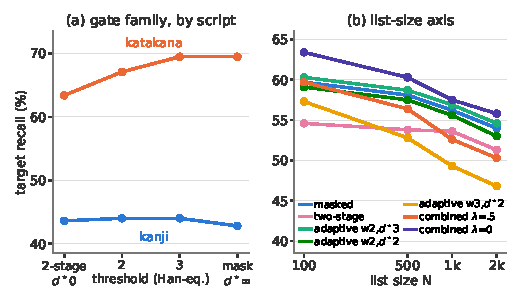
\includegraphics[width=0.98\columnwidth]{figs/fig2_regimes3.pdf}
\caption{Gate-family regimes. (a)~Threshold sweep at matched weight ($w{=}2$, $N{=}1000$); each endpoint degrades in the band the other protects. (b)~Effect of distractor list-size scaling on recall.}
\label{fig:regimes}
\end{figure}


Fig. 2a sweeps the gate threshold at matched weight between the two published endpoints, each of which degrades in the band the other protects. At $d^\star$=0 (two-stage) the entry band is unprotected and katakana recall falls from 69.5\% to 63.4\%; whereas at $d^\star$=$\infty$ (masked) the deep band is capped and kanji recall falls from 44.0\% to 42.8\%. Script determines which band a target occupies, and the benchmark stratifies by it; two-character targets accumulate too little bias for the gate to matter, and all surface configurations converge on them. An intermediate threshold recovers both maxima at once. At $d^\star$=3 the adaptive gate matches the masked endpoint on katakana (69.5\%) and exceeds both on kanji (44.0\% against 43.6\% and 42.8\%), collapsing in neither band.

The effect of distractors is evident as lists scale (Fig. 2b). At most a few of the N listed words occur in any utterance, so as N grows the model more often emits a character opening some listed word that was not spoken, and the automaton spends more of each utterance in spurious partial matches. Such a match pushes toward a wrong continuation, and completes into an insertion, so recall decays everywhere and precision decays faster. How fast depends on push magnitude rather than on the gate. Over a twentyfold increase in N, adaptive at $w$=3 loses 10.5 points of recall and falls to 80\% precision, while every $w$=2 configuration caps losses at 3 to 6 points, and holds precision above 95\%. A smaller $w$ cuts spurious overwrites before rescues, since genuine corrections need only a small push. Delaying the threshold cannot substitute, moving recall by 1 to 3 points where the weight moves 6 to 10, which corroborates the per-scale weight re-tuning in \cite{andrusenko2025turbobias}. The same sensitivity appears across architectures, where OWSM's multi-character pieces deliver several characters of push in one emission and corrupt the hypothesis outright, inflating it to 1.88 times the reference length.


% Scale then decides how much push a list can absorb (Fig. 2b). Over a twentyfold increase in N the masked and adaptive configurations lose 5.7 points of recall, while the ZH-frozen w=3 loses 10.5 with precision falling from 98\% to 80\%, and the $\lambda$=0.5 combination falls from 96\% to 69\%. The two gate parameters are not interchangeable. Raising $w$from 2 to 3 costs 6.3 points of recall at $d^\star$=2 and 10.1 at $d^\star$=3, with precision falling 12 to 14 points in both cases, whereas raising $d^\star$ from 2 to 3 gains 1.3 points at w=2 and loses 2.5 at w=3. The weight dominates, and a later threshold helps only where the push is already bounded, which corroborates the per-scale weight retuning reported in [13]. The same sensitivity appears across architectures, where OWSM's multi-character pieces let one emission advance several characters of a match and the uncapped push then corrupts the hypothesis, inflating it to 1.88 times the reference length and displacing listed words that unbiased decoding had recovered.

% Scale then decides how much push a list can absorb (Fig. 2b). Over a twentyfold increase in N the masked and adaptive configurations lose 5.7 points of recall, with the w=3 loses 10.5 with precision falling from 98\% to 80\%, and the λ=0.5 combination falls from 96\% to 69\%. Reducing the weight recovers most of that loss, corroborating the per-scale retuning reported in [13]. The same sensitivity appears across architectures, where OWSM's multi-character pieces let one emission advance several characters of a match and the uncapped push then corrupts the hypothesis, inflating it to 1.88 times the reference length and displacing listed words that unbiased decoding had recovered.

% Fig. 2a sweeps the gate family from one published parent to the other at matched weight, split by target script. Each endpoint fails in its own band: two-stage (d*=0) leaves the entry band unprotected and loses katakana targets (69.5 → 63.4 on JSUT), mask (d*=∞) caps the deep band and loses kanji (44.0 → 42.8), and d*=3 satisfies both scripts at once. Length tells the same story in the other direction: 2-character targets complete inside the entry band, so every surface gate ties on them and only the reading channel moves that cell (§4v2.3). Weight, not gate, is the fragile axis — and the two parameters disentangle. Holding d*=2 fixed, raising $w$from 2 to 3 costs 6.3 / 0.6pp recall (katakana −12.6 / −8.4) with precision falling 94.9→82.5 / 99.1→96.3; holding w=2 fixed, raising d* from 2 to 3 gains 1.3 / 0.8pp at unchanged precision. The damage is the weight's, concentrated in the deep band on long targets — the per-scale downsweep [13] also documents, and the mask endpoint is immune to it. With the weight matched and d*=3, one fixed setting tracks the mask endpoint within 0.5pp at every list size on both corpora (Fig. 2b, ahead on JSUT throughout), keeps the kanji edge, and its worst-case ZH regret is 2.6 R1 against ≈9 for the best fixed parent: the claim is tuning-freeness as minimax regret, not per-cell wins. Fig. 2b also carries the scale axis: over a 20× list growth the bounded configurations decay gently (mask −5.7 / −3.0pp; two-stage gentlest at −3.3 / −1.2) while w=3 loses 10.5pp with precision falling 98 → 80, and fusion is the best small-list configuration (+3.7 over mask at N=100) but the fastest-decaying, its precision collapsing 96 → 69 (§4v2.3). The tokenizer axis completes the picture: on OWSM's multi-character vocabulary, mask carries over (+13.1 / +21.3pp at P ≥ 93.8) while two-stage collapses outright on both sets (132\% / 155\% CER, recall below greedy). Unbounded deep-band pushes fail on three independent axes — list scale, data regime, tokenizer granularity — and bounded ones survive all three.



%The two regime axes of the gate family (target recall, \%).
% (a)~Sweeping the threshold $d^\star$ at matched weight traces the family from
% one published parent to the other: the two-stage endpoint leaves the entry
% band unprotected and loses katakana targets, the mask endpoint caps the deep
% band and loses kanji targets, and $d^\star{=}3$ reconciles both scripts.
% (b)~List-size axis, both corpora: bounded configurations decay gently over a
% 20$\times$ list growth, while $w{=}3$ and fusion also lose precision at scale
% (98$\to$80 and 96$\to$69 on JSUT); fusion is the best small-list configuration,
% crossing below mask between $N{=}500$ and $1000$.

% Fig. 2a sweeps the family between its parents at matched weight: two-stage leaves the entry band open and loses katakana (69.5 → 63.4 JSUT), mask caps the deep band and loses kanji, and d*=3 satisfies both scripts; 2-character targets complete inside the entry band, so all surface gates tie there and only the reading channel moves that cell (§4v2.3). The two axes disentangle: at fixed d*=2, raising $w$ 2→3 costs 6.3 / 0.6pp (katakana −12.6 / −8.4, precision −12.4 / −2.8); at fixed w=2, raising d* 2→3 gains 1.3 / 0.8pp at unchanged precision — the damage is the weight's, concentrated in the deep band, the per-scale downsweep [13] also documents; the mask endpoint is weight-robust. The matched setting (w2, d*3) tracks mask within 0.5pp at every N on both corpora (Fig. 2b), leads JSUT throughout, and its worst-case ZH regret is 2.6 R1 against ≈9 for the best fixed parent: tuning-freeness as minimax regret. At scale, bounded configurations decay gently (mask −5.7 / −3.0pp over 20×, two-stage least) while w3 loses 10.5pp with precision 98→80 and fusion decays fastest (96→69, §4v2.3); on OWSM's multi-character vocabulary mask carries over (+13.1 / +21.3pp) while two-stage collapses (132\% / 155\% CER). Unbounded deep-band pushes fail on three independent axes — scale, regime, tokenizer granularity — and bounded ones survive all three.



\subsection{Reading-space matching and combination}
Among occurrences the surface decode misses, the proportion whose reading is nevertheless present is 72\% on NE-dense Aishell and 31\% and 18\% on JSUT and CV. The gap separates two kinds of miss. Rare proper nouns, which dominate the JA sets, are misheard outright, whereas orthographic variants are heard correctly but misspelled, the model writing 理屈 for the listed 理窟 and 肩透かし for 肩すかし. Reading-space matching hence addresses spelling rather than recognition errors, which is why it trails surface matching on these sets and why its distinct contribution lies in that second class. For 27 listed words on Aishell, 20 on JSUT and 88 on CV, surface biasing recovers no occurrence, while reading-space matching recovers 31 of 32, all 22, and 131 of 353 respectively. Its gains concentrate on short kanji targets, the condition where all surface gates tie, and are absent on long katakana names, where reading and surface channels coincide.

% Among occurrences the surface decode misses, the proportion whose reading is nevertheless present is 72\% on NE-dense Aishell and 31\% and 18\% on JSUT and CV. The gap separates two kinds of miss. For orthographic variants, like the listed 理窟 which the model writes as the standard 理屈, reading-space matching recovers 14 of 20 occurrences whereas surface biasing recovers none. The rare proper nouns that dominate the JA sets are instead misheard outright. Reading-space matching hence addresses spelling rather than recognition errors, which is why it trails surface matching there. Its gains concentrate on short kanji targets, the condition where all surface gates tie, and are absent on long katakana names, where reading and surface channels coincide. 

Because they miss different occurrences, combining surface and reading channels matches or improves on either alone across all datasets. Whenever both channels push the same token, $\lambda$ adds a share of the weaker score, treating agreement as evidence. As N grows both automata are usually inside some partial match, so a token advancing both signals coincidence more often than agreement. Taking the maximum ($\lambda$=0) ignores the weaker channel altogether, and matches or exceeds $\lambda$>0 at every list size on both corpora while restoring precision (63.4\% at 97.3\% against 59.7\% at 95.5\% on JSUT). Loosening the match itself degrades results; admitting fuzzy pinyin at equal credit was found to lower every metric, since fuzzy transitions move the automaton off the true path as readily as onto it. On WenetSpeech, frequency damping cuts excess insertions from 714 to 304 and raises precision from 96.9\% to 98.6\% at a cost of 0.2 points of recall; on the rare-entity Aishell list it cuts them from 19 to 8, target rarity having already kept the count low.


\section{Conclusion}
We present boundary-free contextual biasing for frozen CTC models, where a character automaton exposes match depth, unifying two gating mechanisms that suit different regimes, and a per-mora or syllable reading state that recovers homophone errors. Combining the two never loses recall against the gate alone and adds up to 3 points. It reaches 66.5\% R1 recall on Aishell-1 NE, above a trained baseline, transfers to WenetSpeech and OWSM unretuned, and gains 25 points on the JA benchmark we release. List composition determines which configuration wins, gains decay as lists grow because push magnitude is a tuned constant, and multi-character vocabularies still need the masked endpoint. Both mechanisms assume dense scripts. In a language like Thai where a character carries less evidence, partial matches are common and depth accrues credit too fast, while a phonemic orthography leaves little for reading-space matching; the schedule would need recalibrating in information units.

% We present boundary-free contextual biasing for frozen CTC models, where a character automaton exposes match depth, unifying two gating mechanisms that suit different regimes, and a per-mora or per-syllable reading state that recovers homophone errors. Fusing the two is complementary, within 1.7 points of the best configuration on every evaluation. Training-free and single-pass, it reaches 66.5\% recall on Aishell-1 NE's R1 subset, above a trained baseline, transfers to WenetSpeech and OWSM unretuned, and gains 22 and 25 points on the JA benchmark we release. List composition determines which configuration wins, gains decay as lists grow because push magnitude is a tuned constant, and multi-character vocabularies still require the masked endpoint. Both mechanisms assume dense scripts. In Thai a character carries less evidence, so spurious partial matches are common and depth accrues credit too fast, while a phonemic orthography leaves reading-space matching little to recover; the schedule would need recalibrating in information rather than character units.

% One setting is stable across all three axes. At w=2 and d*=3 the adaptive gate tracks the masked endpoint within 0.5 points at every list size on both corpora, at a worst-case regret of 2.6 points of R1 recall on ZH against approximately 9 for the best fixed parent. It wins no cell outright, and its value is invariance to a regime unknown at deployment time.

% Character-level matching does not improve recognition by itself, as surface and token-level matching tie once the token baseline is built correctly, which required resolving three tokenizer encoding conventions. It is instead correct by construction, and it exposes two quantities that word-level biasing cannot: per-character match depth, on which the gate switches, and per-mora state, on which reading-space matching operates. Both mechanisms are decode-only, add constant work per frame, and require no modification of the acoustic model, so they apply to any frozen CTC system. Three limitations bound the results. Reading-space matching addresses homophone and orthographic-variant errors only; misrendered readings are unreachable by construction. The per-script information weights are a two-entry approximation to a corpus surprisal table. The fixed gate setting holds per tokenizer class, since multi-character vocabularies require the bounded endpoint. We release the benchmark, lists, annotations and verification suite so that the regime analysis, and not only the headline results, can be reproduced.

% \section{Formatting your paper}
% \label{sec:format}

% All printed material, including text, illustrations, and charts, must be kept
% within a print area of 7 inches (178 mm) wide by 9 inches (229 mm) high. Do
% not write or print anything outside the print area. The top margin must be 1
% inch (25 mm), except for the title page, and the left margin must be 0.75 inch
% (19 mm).  All {\it text} must be in a two-column format. Columns are to be 3.39
% inches (86 mm) wide, with a 0.24 inch (6 mm) space between them. Text must be
% fully justified.

% \section{PAGE TITLE SECTION}
% \label{sec:pagestyle}

% The paper title (on the first page) should begin 1.38 inches (35 mm) from the
% top edge of the page, centered, completely capitalized, and in Times 14-point,
% boldface type.  The authors' name(s) and affiliation(s) appear below the title
% in capital and lower case letters.  Papers with multiple authors and
% affiliations may require two or more lines for this information. Please note
% that papers should not be submitted blind; include the authors' names on the
% PDF.

% \section{TYPE-STYLE AND FONTS}
% \label{sec:typestyle}

% To achieve the best rendering both in printed proceedings and electronic proceedings, we
% strongly encourage you to use Times-Roman font.  In addition, this will give
% the proceedings a more uniform look.  Use a font that is no smaller than nine
% point type throughout the paper, including figure captions.

% In nine point type font, capital letters are 2 mm high.  {\bf If you use the
% smallest point size, there should be no more than 3.2 lines/cm (8 lines/inch)
% vertically.}  This is a minimum spacing; 2.75 lines/cm (7 lines/inch) will make
% the paper much more readable.  Larger type sizes require correspondingly larger
% vertical spacing.  Please do not double-space your paper.  TrueType or
% Postscript Type 1 fonts are preferred.

% The first paragraph in each section should not be indented, but all the
% following paragraphs within the section should be indented as these paragraphs
% demonstrate.

% \section{MAJOR HEADINGS}
% \label{sec:majhead}

% Major headings, for example, "1. Introduction", should appear in all capital
% letters, bold face if possible, centered in the column, with one blank line
% before, and one blank line after. Use a period (".") after the heading number,
% not a colon.

% \subsection{Subheadings}
% \label{ssec:subhead}

% Subheadings should appear in lower case (initial word capitalized) in
% boldface.  They should start at the left margin on a separate line.
 
% \subsubsection{Sub-subheadings}
% \label{sssec:subsubhead}

% Sub-subheadings, as in this paragraph, are discouraged. However, if you
% must use them, they should appear in lower case (initial word
% capitalized) and start at the left margin on a separate line, with paragraph
% text beginning on the following line.  They should be in italics.

% \section{PRINTING YOUR PAPER}
% \label{sec:print}

% Print your properly formatted text on high-quality, 8.5 x 11-inch white printer
% paper. A4 paper is also acceptable, but please leave the extra 0.5 inch (12 mm)
% empty at the BOTTOM of the page and follow the top and left margins as
% specified.  If the last page of your paper is only partially filled, arrange
% the columns so that they are evenly balanced if possible, rather than having
% one long column.

% In LaTeX, to start a new column (but not a new page) and help balance the
% last-page column lengths, you can use the command ``$\backslash$pagebreak'' as
% demonstrated on this page (see the LaTeX source below).

% \section{PAGE NUMBERING}
% \label{sec:page}

% Please do {\bf not} paginate your paper.  Page numbers, session numbers, and
% conference identification will be inserted when the paper is included in the
% proceedings.

% \section{ILLUSTRATIONS, GRAPHS, AND PHOTOGRAPHS}
% \label{sec:illust}

% Illustrations must appear within the designated margins.  They may span the two
% columns.  If possible, position illustrations at the top of columns, rather
% than in the middle or at the bottom.  Caption and number every illustration.
% All halftone illustrations must be clear black and white prints.  Colors may be
% used, but they should be selected so as to be readable when printed on a
% black-only printer.

% Since there are many ways, often incompatible, of including images (e.g., with
% experimental results) in a LaTeX document, below is an example of how to do
% this \cite{Lamp86}.

% \section{FOOTNOTES}
% \label{sec:foot}

% Use footnotes sparingly (or not at all!) and place them at the bottom of the
% column on the page on which they are referenced. Use Times 9-point type,
% single-spaced. To help your readers, avoid using footnotes altogether and
% include necessary peripheral observations in the text (within parentheses, if
% you prefer, as in this sentence).

% % Below is an example of how to insert images. Delete the ``\vspace'' line,
% % uncomment the preceding line ``\centerline...'' and replace ``imageX.ps''
% % with a suitable PostScript file name.
% % -------------------------------------------------------------------------
% \begin{figure}[htb]

% \begin{minipage}[b]{1.0\linewidth}
%   \centering
%   \centerline{\includegraphics[width=8.5cm]{image1}}
% %  \vspace{2.0cm}
%   \centerline{(a) Result 1}\medskip
% \end{minipage}
% %
% \begin{minipage}[b]{.48\linewidth}
%   \centering
%   \centerline{\includegraphics[width=4.0cm]{image3}}
% %  \vspace{1.5cm}
%   \centerline{(b) Results 3}\medskip
% \end{minipage}
% \hfill
% \begin{minipage}[b]{0.48\linewidth}
%   \centering
%   \centerline{\includegraphics[width=4.0cm]{image4}}
% %  \vspace{1.5cm}
%   \centerline{(c) Result 4}\medskip
% \end{minipage}
% %
% \caption{Example of placing a figure with experimental results.}
% \label{fig:res}
% %
% \end{figure}


% % To start a new column (but not a new page) and help balance the last-page
% % column length use \vfill\pagebreak.
% % -------------------------------------------------------------------------
% %\vfill
% %\pagebreak

% \section{COPYRIGHT FORMS}
% \label{sec:copyright}

% You must submit your fully completed, signed IEEE electronic copyright release
% form when you submit your paper. We {\bf must} have this form before your paper
% can be published in the proceedings.

% \section{RELATION TO PRIOR WORK}
% \label{sec:prior}

% The text of the paper should contain discussions on how the paper's
% contributions are related to prior work in the field. It is important
% to put new work in  context, to give credit to foundational work, and
% to provide details associated with the previous work that have appeared
% in the literature. This discussion may be a separate, numbered section
% or it may appear elsewhere in the body of the manuscript, but it must
% be present.

% You should differentiate what is new and how your work expands on
% or takes a different path from the prior studies. An example might
% read something to the effect: "The work presented here has focused
% on the formulation of the ABC algorithm, which takes advantage of
% non-uniform time-frequency domain analysis of data. The work by
% Smith and Cohen \cite{Lamp86} considers only fixed time-domain analysis and
% the work by Jones et al \cite{C2} takes a different approach based on
% fixed frequency partitioning. While the present study is related
% to recent approaches in time-frequency analysis [3-5], it capitalizes
% on a new feature space, which was not considered in these earlier
% studies."

\vfill\pagebreak

% \section{REFERENCES}
% \label{sec:refs}

% List and number all bibliographical references at the end of the
% paper. The references can be numbered in alphabetic order or in
% order of appearance in the document. When referring to them in
% the text, type the corresponding reference number in square
% brackets as shown at the end of this sentence \cite{C2}. An
% additional final page (the fifth page, in most cases) is
% allowed, but must contain only references to the prior
% literature.

% References should be produced using the bibtex program from suitable
% BiBTeX files (here: strings, refs, manuals). The IEEEbib.bst bibliography
% style file from IEEE produces unsorted bibliography list.
% -------------------------------------------------------------------------
\bibliographystyle{IEEEbib}
\bibliography{refs}

\end{document}
